\documentclass[a4paper]{article}
\usepackage[english]{babel}
\usepackage[utf8]{inputenc}
\usepackage{graphicx}
\usepackage{hyperref}

\title{Understanding The Things Network's Software}

\author{Mohd Thaqif ABDULLAH HASIM}

\date{\today}

\begin{document}
\maketitle

\begin{abstract}
During a full time preparatory week, I need to have a good understanding of the software provided by The Things Network in order to establish a LoRa network for the use of IoT.
\end{abstract}

\section{Architecture of TTN}
\label{sec:introduction}

Data sent by the things (Nodes/devices) to the application will be routed through different routing service components. The gateway will act as a router by forwarding the packets sent by the devices to The Things Network. 
The Things Network is positioned between the gateways and the applications (see the figure below) and takes care of these routing and processing steps.

\begin{figure}[h]
\centering
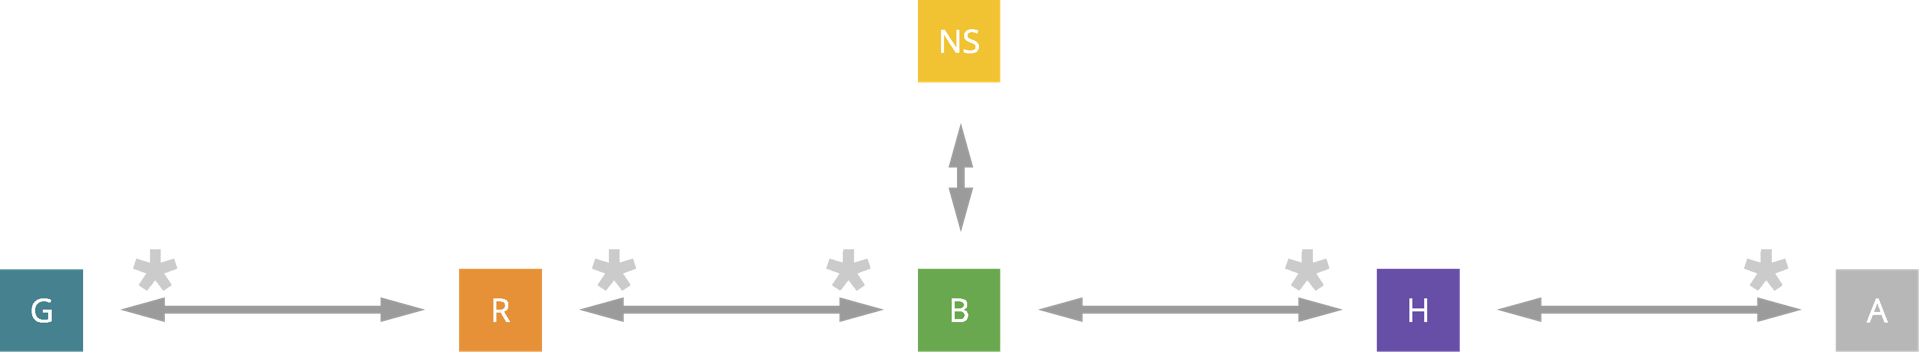
\includegraphics[width=1\textwidth]{Routing-Services.png}
\caption{\label{fig:Routing-Services}The Things Network’s different routing service components:
Gateway, Router, Broker, NetworkServer, Handler and Application}
\end{figure}

Nodes (N in the top Figure) broadcast LoRaWAN messages over the LoRa radio protocol. 
These messages are received by a number of Gateways (G). 
The Gateway is a piece of hardware that forwards radio transmissions to the backend. 
It is connected to one Router (R). 
The Router is responsible for managing the gateway's status and for scheduling transmissions. 
Each Router is connected to one or more Brokers (B). 
Brokers are the central part of The Things Network. 
Their responsibility is to map a device to an application, to forward uplink messages to the correct application and to forward downlink messages to the correct Router (which forwards them to a Gateway). 
The Network Server (NS) is responsible for functionality that is specific for LoRaWAN. 
A Handler (H) is responsible for handling the data of one or more Applications (A). 
To do so, it connects to a Broker where it registers applications and devices. 
The Handler is also the point where data is encrypted or decrypted.

\begin{flushleft}
The are two options to deploy a network :
\end{flushleft}
 \begin{enumerate}
  \item Public Community Network
  \item Private Network
 \end{enumerate}
 
We can run The Things Network on our own server by downloading TTN's open source routing services from GitHub 
\url{https://github.com/TheThingsNetwork/ttn}. I have downloaded it and tried to run TTN's routing services on my computer.
I have passed the first step which is \textbf{to prepare the development environment} by installing some packages.
Next step is \textbf{to set up TTN's backend for development}. At this step, after installing the dependencies for the development,
the tests ran fail and the next steps can't be proceeded.

After visiting the TTN's FAQ, it is recommanded to just use the public community network, as this will save a lot of time.
We can run a private deployment TTN's open source routing services if we know what we are doing.

\section{Gateway}

By using the pubic community network, I can concentrate on how to set up the gateway and make it communicate with TTN's backend.
LIG owns some Kerlink gateways that need to be configured. A documentation on how to configure this type of gateway can be consulted at 
\url{https://www.thethingsnetwork.org/wiki/Hardware/Gateways/Kerlink}

\subsection{Configure the Gateway}
\href{https://github.com/TheThingsNetwork/kerlink-station-firmware}{Kerlink's repository on GitHub} contains the software en tools to use the Kerlink Gateway with TTN. 
\newline 

Steps of the configuration :
\begin{enumerate}
 \item Download TTN's 
 \href{https://github.com/TheThingsNetwork/kerlink-station-firmware/raw/master/dota/dota_thethingsnetwork_v1.3_EU.tar.gz}{patch/update file}
 and \href{https://github.com/TheThingsNetwork/kerlink-station-firmware/raw/master/dota/produsb.zip}{produsb.zip}
 \item Install the patch/update downloaded :
 \begin{enumerate}
  \item Extract the compressed files downloaded onto on empty USB flash drive formatted in \textit{FAT-32}.Make sure there is no \textit{.log} file.
  \item Plug the USB flash drive into the gateway.
  \item Wait for 5 min. During this time the gateway will reboot itself.
  \item Unplug the key and check that a \textit{.log} file has appeared. The file should contain the following text \textit{WirmaV2 0x080XXXXX updated}. This log file prevents any further installation on the gateways to avoid cyclic reboots.
To redo the update on same gateway, remove this log file from the flash drive reinsert it into the gateway USB. This is not needed if you update another gateway.
 \end{enumerate}
 \item Logon to the gateway by using the SSH protocol, run 
 \newline \framebox[1.1\width]{ssh root@\textit{Gateway's IP}}\par
 \item At your firewall system make sure the external IP-address used will map port 1700 to the internal IP-address of the gateway. This is needed when using NAT for internal IP-address translation.
 \item Use the following command on the gateway to check whether data is being sent and received: 
 \newline \framebox[1.1\width]{tcpdump -i eth0 -n -vvvX host \textit{hostname}}\par
 \item There is a documentation on \href{https://github.com/swiatecki/IoTPublic/blob/master/howto.md}{how to regain \textit{root} access on Kerlink}
\end{enumerate}

\subsection{Connect the Gateway to TTN's backend}
\subsubsection{Server Address}
Choose the router instance depanding on the region. 
\newline \framebox[1.1\width]{router.eu.thethings.network \#EU 433 and EU 863-870}\par

\subsubsection{Configuring the Gateway}
\textit{NOTE: Please use a packet forwarder based on version 2.2.x. The new lora\_pkt\_fwd version 3.0.0 is not supported yet}\par
In the local\_conf.json of the packet forwarder, update the fields server\_address as follows:

\begin{figure}[h]
\centering
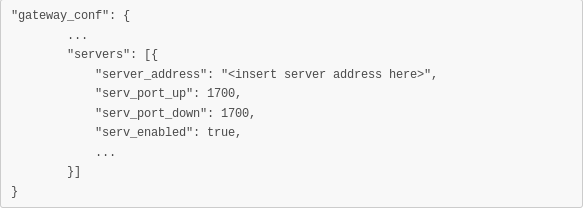
\includegraphics[width=1\textwidth]{config_gateway.png}
\caption{\label{fig:config_gateway}}
\end{figure}

\subsubsection{Checking Connectivity}
\begin{enumerate}
 \item Gateway communicates with the routers via an UDP connection on port 1700; So if we listen to this port we should see packets being transferred.
\newline \framebox[1.1\textwidth]{\textit{sudo tcpdump -AUq port 1700}}\par
\item The packet forwarder periodically writes its status to a log file located at: /var/log/syslog
\newline \framebox[1.1\textwidth]{\textit{sudo tail -f /var/log/syslog}}\par
\end{enumerate}


\end{document}
